%Yuga_counter_example_recovery.tex




\documentclass{standalone}
% newcommands.tex

\newcommand{\enq}{\texttt{enq}}
\newcommand{\deq}{\texttt{deq}}
\newcommand{\pput}{\texttt{PUT}}
\newcommand{\get}{\texttt{GET}}
\newcommand{\vs}{\texttt{vis}}
\newcommand{\so}{\texttt{so}}
\newcommand{\arb}{\texttt{ar}}
\newcommand{\rf}{\texttt{rf}}

% example
\newcommand{\po}[2]{\draw [->, thick] (#1) to node[above] {\Large{\so}} (#2);}
\newcommand{\pva}[2]{\draw [->, thick] (#1) to node[above] {$\Large{\so},\Large{\vs},\Large{\arb}$} (#2);}
\newcommand{\pbva}[2]{\draw [->, thick] (#1) to node[above] {$\Large{\so}$} node[below] {$\Large{\vs},\Large{\arb}$} (#2);}
\newcommand{\pv}[2]{\draw [->, thick] (#1) to node[above] {\Large{\so}} node[below] {\Large{\vs}} (#2);}
\newcommand{\evis}[2]{\draw [->, thick] (#1) to node[above, sloped, near end] {\Large{\vs}} (#2);}
\newcommand{\mvis}[2]{\draw [->, thick] (#1) to node[above, sloped] {\Large{\vs}} (#2);}
\newcommand{\ar}[2]{\draw [->, thick, allow upside down] (#1) to node[above, sloped] {\Large{\arb}} (#2);}
\newcommand{\va}[2]{\draw [->, thick, allow upside down] (#1) to node[above, sloped] {$\Large{\vs},\Large{\arb}$} (#2);}
\newcommand{\vab}[2]{\draw [->, thick, allow upside down] (#1) to node[below, sloped, near end] {$\Large{\vs},\Large{\arb}$} (#2);}
\newcommand{\vae}[2]{\draw [->, thick, allow upside down] (#1) to node[above, sloped, near end] {$\Large{\vs},\Large{\arb}$} (#2);}
\newcommand{\vas}[2]{\draw [->, thick, allow upside down] (#1) to node[sloped, near start, above] {$\Large{\vs},\Large{\arb}$} (#2);}

% serialization
\newcommand{\scc}[2]{\draw [->, very thick] (#1) to (#2);}
\newcommand{\rva}[2]{\draw [->, thick, allow upside down] (#1) to node[above, sloped] {$\Large{\rf},\Large{\vs},\Large{\arb}$} (#2);}
\newcommand{\rvb}[2]{\draw [->, thick, allow upside down] (#1) to node[below, sloped] {$\Large{\rf},\Large{\vs},\Large{\arb}$} (#2);}


\usepackage{tikz}
\usetikzlibrary{shapes, positioning, arrows.meta, decorations.pathmorphing}

\begin{document}

    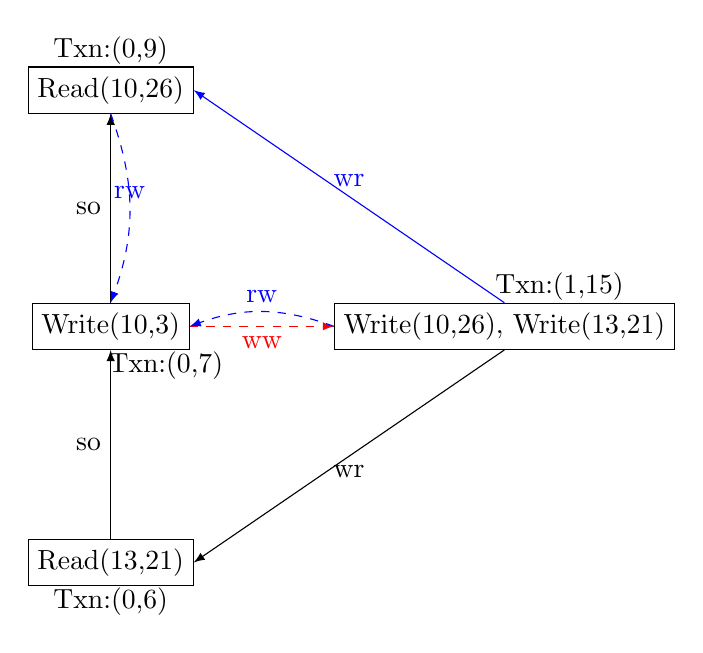
\begin{tikzpicture}[model/.style = {draw, minimum size = 15pt},  node distance = 0.5cm and 1.5cm]
        \node[model] (07) at (0,0) {Write(10,3)};
        \node (textof07) at (0.7,-0.5) {Txn:(0,7)};
        \node[model] (06) at (0,-3) {Read(13,21)};
        \node (textof06) at (0,-3.5) {Txn:(0,6)};
        \node[model] (115) at (5,0) {Write(10,26), Write(13,21)};
        \node (textof115) at (5.7,0.5) {Txn:(1,15)};
        \node[model] (09) at (0,3) {Read(10,26)};
        \node (textof09) at (0,3.5) {Txn:(0,9)};
        
        \path[dashed, -latex, color=red] (07.east) edge node[below] {ww} (115.west); 
        \path[-latex] (06.north) edge node[left] {so} (07.south); 
        \path[-latex] (115.south) edge node[below] {wr} (06.east); 
        \path[-latex] (07.north) edge node[left] {so} (09.south); 
        \path[-latex,color=blue] (115.north) edge node[above] {wr} (09.east); 
        \path[dashed, -latex,color=blue] (09.south) edge [out=-70,in=70] node[above] {rw} (07.north); 
        \path[dashed, -latex,color=blue] (115.west) edge [out=160,in=20] node[above] {rw} (07.east); 
    \end{tikzpicture}
\end{document}